\documentclass[12pt]{article}

\usepackage{graphicx}
\usepackage{amsmath}
\usepackage{mathtools}
\usepackage{tikz}
\usepackage{pgf-pie}
\usepackage{tikz-cd}
\usetikzlibrary{arrows}
\usepackage{cancel}
\usepackage{setspace}
\usepackage{indentfirst}
\usepackage{afterpage}
\usepackage{caption}
\usepackage[raggedrightboxes]{ragged2e}
\usepackage{tabularx}
\usepackage{bbding}
\usepackage{pifont}
\usepackage{textcomp}
\usepackage{xspace}
\usepackage{verbatim}
\usepackage{wrapfig}

\title{Multiplication Course\\
\begin{center}

\includegraphics[width=4em]{ApS_logo.png}
\end{center}
\begin{normalsize}Applied Scholastics, Ferndale \end{normalsize}}
\author{}
\date{}

\begin{document}
\maketitle

\section*{Multiplication}

\paragraph{Multiply}
Multiply is a Latin word. Multi- means many, and -ply means fold, so multiply means folded many times. Multiply means to add a number to itself many times.\\

\begin{enumerate}

\item What does multiply mean, in your own words?
\item Use the word 'multiply' in 3 sentences.

\paragraph{Times}
Multiplication is also called times, because multiplication means adding a number to itself many times.\\

\item What does times mean, in your own words?
\item Use the word 'times' in 3 sentences.

\paragraph{Times Symbol}
The times symbol is $\times$ :\\

$\overbrace{8+8+8+8}^{\textrm{8 added to itself 4 times}}= 8 \times 4 = 32$\\

Sometimes a raised dot ($\text{ }\cdot$\text{ })is used instead of the times symbol because $\times$ can be confused for the letter x, and because it is shorter. $3 \cdot 4$ means $3 \times 4$.\\

In more advanced maths, the times symbol is often just left out. If two things are next to each other in a maths statement it is assumed that times is meant.\\

\paragraph{Multiplicand}
The number being multiplied is called the multiplicand, which is Latin for "to be multiplied."\\

\item What does multiplicand mean, in your own words?
\item Use the word 'multiplicand' in a sentence.

\paragraph{Multiplier}
The number it is being multiplied by is called the multiplier.\\

\item What does multiplier mean, in your own words?
\item Use the word 'multiplier' in a sentence.

\paragraph{Product}
The result of multiplying is called the product.\\

\item What does product mean, in your own words?
\item Use the word 'product' in a sentence.

$$\text{Multiplicand}\times \text{Multiplier} = \text{Product.}$$

\section*{Commutative Law of Multiplication}

To commute means to go back and forth between two places, like when people commute to and from their work each day. Commutative means that something goes back and forth.\\

\item What does commute mean, in your own words?
\item Use commute in a sentence.
\item What does commutative mean, in your own words?
\item Use commutative in a sentence.

The commutative law of multiplication is that multiplication is commutative because numbers can multiplied be in any order and the product will be the same.\\

It is also sometimes called the commutative property of multiplication.\\

$$8 \times 7 = 7\times 8$$
$$22 \times 42 = 42 \times 22$$

\item Explain in your own words why multiplication is said to be commutative.

\section*{Associative Law of Multiplication}
To associate means to be in a group with others. An associate is another word for someone you spend time with. Associative means someone or something that likes to associate.\\

\item What does associate mean, in your own words?
\item Use associate in a sentence.
\item What does associative mean, in your own words?
\item Use associative in a sentence.

Multiplication is said to be associative because the numbers can be put into different groups, using brackets, and the product is the same. It doesn't matter which part is calculated first. That means that problems can be rearranged to make them easier to work out.\\

$$(1\times2)\times3=1\times(2\times3)$$
$$(11\times3)\times4=11\times(3\times4)$$

\item Explain in your own words why multiplication is said to be associative.

\section*{The Multiplicative Identity}
Identity means who someone is. Another meaning of identity is where two things that are identical, being exactly the same, are said to be an identity.\\

\item What is an identity, in your own words?
\item Think of two things that are an identity.

1 is called the additive identity because a number doesn’t change when multiplied by 1. Any number equals itself multiplied by 1. This fact is used in later mathematics.

\item In your own words, why is 1 called the multiplicative identity?

\section*{Skip Counting}
\paragraph{Multiples}
Learning skip counting is the first step in learning to multiply. These are the multiples of a number.\\

Practice until you can skip count all the way to 100 for any number from 2 to 10,  without looking.\\

\item Practice counting by twos all the way to 100:\\
2, 4, 6, 8, 10, 12, 14, 16, 18, 20, 22, 24, 26, 28, 30, 32, 34, 36, 38, 40, 42, 44, 46, 48, 50, 52, 54, 56, 58, 60, 62, 64, 66, 68, 70, 72, 74, 76, 78, 80, 82, 84, 86, 88, 90, 92, 94, 96, 98, 100.

\begin{center}
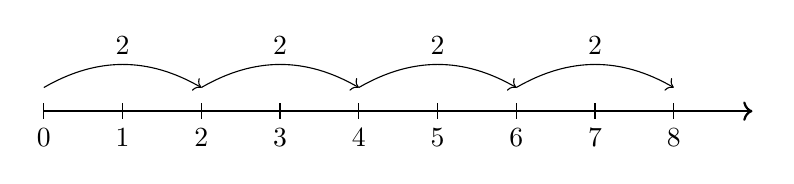
\begin{tikzpicture}
\draw[thick, ->] (0,0) -- (9,0) node[below] {$\ $};
\foreach \n in {0,1,2,3,4,5,6,7,8} {\draw (\n,0.1) -- (\n,-0.1) node[below] {$\n$};}
\draw[->, bend left=30] (0,0.3) to node[above] {$2$} (2,0.3);
\draw[->, bend left=30] (2,0.3) to node[above] {$2$} (4,0.3);
\draw[->, bend left=30] (4,0.3) to node[above] {$2$} (6,0.3);
\draw[->, bend left=30] (6,0.3) to node[above] {$2$} (8,0.3);
\end{tikzpicture}
\end{center}

\item Practice counting by threes all the way to 100:\\
3, 6, 9, 12, 15, 18, 21, 24, 27, 30, 33, 36, 39, 42, 45, 48, 51, 54, 57, 60, 63, 66, 69, 72, 75, 78, 81, 84, 87, 90, 93, 96, 99.

\begin{center}
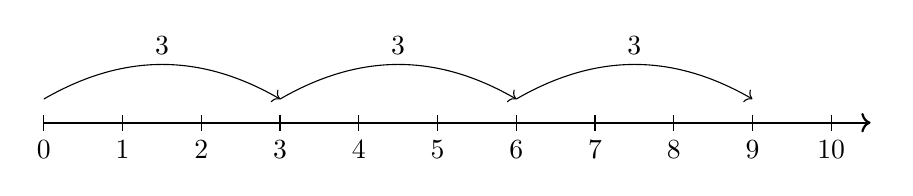
\begin{tikzpicture}
\draw[thick, ->] (0,0) -- (10.5,0) node[below] {$\ $};
\foreach \n in {0,1,2,3,4,5,6,7,8,9,10}
{\draw (\n,0.1) -- (\n,-0.1) node[below] {$\n$};}
\draw[->, bend left=30] (0,0.3) to node[above] {$3$} (3,0.3);
\draw[->, bend left=30] (3,0.3) to node[above] {$3$} (6,0.3);
\draw[->, bend left=30] (6,0.3) to node[above] {$3$} (9,0.3);
\end{tikzpicture}
\end{center}

\item Practice counting by fours all the way to 100:\\
4, 8, 12, 16, 20, 24, 28, 32, 36, 40, 44, 48, 52, 56, 60, 64, 68, 72, 76, 80, 84, 88, 92, 96, 100.

\begin{center}
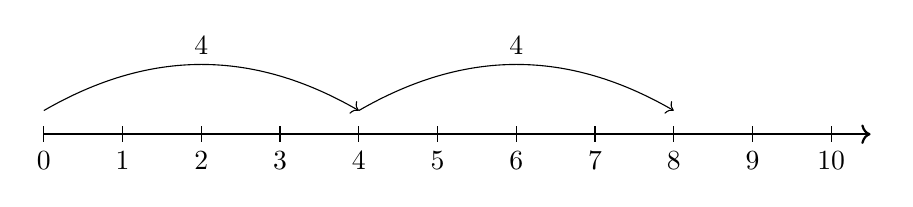
\begin{tikzpicture}
\draw[thick, ->] (0,0) -- (10.5,0) node[below] {$\ $};
\foreach \n in {0,1,2,3,4,5,6,7,8,9,10} {\draw (\n,0.1) -- (\n,-0.1) node[below] {$\n$};}
\draw[->, bend left=30] (0,0.3) to node[above] {$4$} (4,0.3);
\draw[->, bend left=30] (4,0.3) to node[above] {$4$} (8,0.3);
\end{tikzpicture}
\end{center}

\item Practice counting by fives all the way to 100:\\
5, 10, 15, 20, 25, 30, 35, 40, 45, 50, 55, 60, 65, 70, 75, 80, 85, 90, 95, 100.\\

\item Practice counting by sixes all the way to 100:\\
6, 12, 18, 24, 30, 36, 42, 48, 54, 60, 66, 72, 78, 84, 90, 96.\\

\item Practice counting by sevens all the way to 100:\\
7, 14, 21, 28, 35, 42, 49, 56, 63, 70, 77, 84, 91, 98.\\

\item Practice counting by eights all the way to 100:\\
8, 16, 24, 32, 40, 48, 56, 64, 72, 80, 88, 96.\\

\item Practice counting by nines all the way to 100:\\
9, 18, 27, 36, 45, 54, 63, 72, 81, 90, 99.\\

\item Practice counting by tens all the way to 100:\\
10, 20, 30, 40, 50, 60, 70, 80, 90, 100.\\

\item Drill skip counting every day, especially the ones you have trouble with, until you can do them all easily.

\pagebreak

\section*{The Times Table}

\paragraph{Times table up to 10}
Now learn the times table from 1 to 10, by heart.\\

Drilling the times table is best done as part of a group of students, good and loud, but you can do it on your own as well of course.\\

If a teacher is helping then it is a good idea to put up a large copy of the times table and have the teacher lead the group by pointing to each number.\\

\begin{center}
\begin{tabular}{|c||*{10}{c|}}
\hline
$\times$ & 1 & 2 & 3 & 4 & 5 & 6 & 7 & 8 & 9 & 10 \\
\hline\hline
1 & 1 & 2 & 3 & 4 & 5 & 6 & 7 & 8 & 9 & 10 \\
2 & 2 & 4 & 6 & 8 & 10 & 12 & 14 & 16 & 18 & 20 \\
3 & 3 & 6 & 9 & 12 & 15 & 18 & 21 & 24 & 27 & 30 \\
4 & 4 & 8 & 12 & 16 & 20 & 24 & 28 & 32 & 36 & 40 \\
5 & 5 & 10 & 15 & 20 & 25 & 30 & 35 & 40 & 45 & 50 \\
6 & 6 & 12 & 18 & 24 & 30 & 36 & 42 & 48 & 54 & 60 \\
7 & 7 & 14 & 21 & 28 & 35 & 42 & 49 & 56 & 63 & 70 \\
8 & 8 & 16 & 24 & 32 & 40 & 48 & 56 & 64 & 72 & 80 \\
9 & 9 & 18 & 27 & 36 & 45 & 54 & 63 & 72 & 81 & 90 \\
10 & 10 & 20 & 30 & 40 & 50 & 60 & 70 & 80 & 90 & 100 \\
\hline
\end{tabular}
\end{center}

\item Drill the 2-times table:\\

"1 times 2 is 2."\\
"2 times 2 is 4."\\
"3 times 2 is 6."\\
"4 times 2 is 8."\\
"6 times 2 is 12."\\
"7 times 2 is 14."\\
"8 times 2 is 16."\\
"9 times 2 is 18."\\
"10 times 2 is 20."\\

Say the 2-times table out loud, many times, until you can do it easily.\\

\item Drill the 3-times table:\\

"1 times 3 is 3."\\
"2 times 3 is 6."\\
"3 times 3 is 9."\\
"4 times 3 is 12."\\
"5 times 3 is 15."\\
"6 times 3 is 18."\\
"7 times 3 is 21."\\
"8 times 3 is 24."\\
"9 times 3 is 27."\\
"10 times 3 is 30."\\

Say the 3-times table out loud, many times, until you can do it easily.\\

\item Drill the 4-times table:\\

"1 times 4 is 4."\\
"2 times 4 is 8."\\
"3 times 4 is 12."\\
"4 times 4 is 16."\\
"5 times 4 is 20."\\
"6 times 4 is 24."\\
"7 times 4 is 28."\\
"8 times 4 is 32."\\
"9 times 4 is 36."\\
"10 times 4 is 40."\\

Say the 4-times table out loud, many times, until you can do it easily.\\

\item Drill the 4-times table:\\

"1 times 5 is 5."\\
"2 times 5 is 10."\\
"3 times 5 is 15."\\
"4 times 5 is 20."\\
"5 times 5 is 25."\\
"6 times 5 is 30."\\
"7 times 5 is 35."\\
"8 times 5 is 40."\\
"9 times 5 is 45."\\
"10 times 5 is 50."\\

Say the 5-times table out loud, many times, until you can do it easily.\\

\item Drill the 6-times table:\\

"1 times 6 is 6."\\
"2 times 6 is 12."\\
"3 times 6 is 18."\\
"4 times 6 is 24."\\
"5 times 6 is 30."\\
"6 times 6 is 36."\\
"7 times 6 is 42."\\
"8 times 6 is 48."\\
"9 times 6 is 54."\\
"10 times 6 is 60."\\

Say the 6-times table out loud, many times, until you can do it easily.\\

\item Drill the 7-times table:\\

"1 times 7 is 7."\\
"2 times 7 is 14."\\
"3 times 7 is 21."\\
"4 times 7 is 28."\\
"5 times 7 is 35."\\
"6 times 7 is 42."\\
"7 times 7 is 49."\\
"8 times 7 is 56."\\
"9 times 7 is 63."\\
"10 times 7 is 70."\\

Say the 7-times table out loud, many times, until you can do it easily.\\

\item Drill the 8-times table:\\

"1 times 8 is 8."\\
"2 times 8 is 16."\\
"3 times 8 is 24."\\
"4 times 8 is 32."\\
"5 times 8 is 40."\\
"6 times 8 is 48."\\
"7 times 8 is 56."\\
"8 times 8 is 64."\\
"9 times 8 is 72."\\
"10 times 8 is 80."\\

Say the 8-times table out loud, many times, until you can do it easily.\\

\item Drill the 9-times table:\\

"1 times 9 is 9."\\
"2 times 9 is 18."\\
"3 times 9 is 27."\\
"4 times 9 is 36."\\
"5 times 9 is 45."\\
"6 times 9 is 54."\\
"7 times 9 is 63."\\
"8 times 9 is 72."\\
"9 times 9 is 81."\\
"10 times 9 is 90."\\

Say the 9-times table out loud, many times, until you can do it easily.\\

\item Drill the 10-times table:\\

"1 times 10 is 10."\\
"2 times 10 is 20."\\
"3 times 10 is 30."\\
"4 times 10 is 40."\\
"5 times 10 is 50."\\
"6 times 10 is 60."\\
"7 times 10 is 70."\\
"8 times 10 is 80."\\
"9 times 10 is 90."\\
"10 times 10 is 100."\\

Say the 10-times table out loud, many times, until you can do it easily.\\

\item Pick any two numbers, each  from 1 to 10. What is their product?
\item Keep picking random pairs of numbers from 1 to 10 and saying their product until you know all the answers straight away.

\pagebreak

\paragraph{Times Table up to 12}
Now learn the times table for 11 and 12.\\

\begin{center}
\begin{tabular}{|c||c|c|c|c|c|c|c|c|c|c|c|c|}
\hline
$\times$ & 1 & 2 & 3 & 4 & 5 & 6 & 7 & 8 & 9 & 10 & 11 & 12 \\
\hline\hline
1 & 1 & 2 & 3 & 4 & 5 & 6 & 7 & 8 & 9 & 10 & 11 & 12 \\
2 & 2 & 4 & 6 & 8 & 10 & 12 & 14 & 16 & 18 & 20 & 22 & 24 \\
3 & 3 & 6 & 9 & 12 & 15 & 18 & 21 & 24 & 27 & 30 & 33 & 36 \\
4 & 4 & 8 & 12 & 16 & 20 & 24 & 28 & 32 & 36 & 40 & 44 & 48 \\
5 & 5 & 10 & 15 & 20 & 25 & 30 & 35 & 40 & 45 & 50 & 55 & 60 \\
6 & 6 & 12 & 18 & 24 & 30 & 36 & 42 & 48 & 54 & 60 & 66 & 72 \\
7 & 7 & 14 & 21 & 28 & 35 & 42 & 49 & 56 & 63 & 70 & 77 & 84 \\
8 & 8 & 16 & 24 & 32 & 40 & 48 & 56 & 64 & 72 & 80 & 88 & 96 \\
9 & 9 & 18 & 27 & 36 & 45 & 54 & 63 & 72 & 81 & 90 & 99 & 108 \\
10 & 10 & 20 & 30 & 40 & 50 & 60 & 70 & 80 & 90 & 100 & 110 & 120 \\
11 & 11 & 22 & 33 & 44 & 55 & 66 & 77 & 88 & 99 & 110 & 121 & 132 \\
12 & 12 & 24 & 36 & 48 & 60 & 72 & 84 & 96 & 108 & 120 & 132 & 144 \\
\hline
\end{tabular}
\end{center}

\item Start by learning to count by elevens to 100:
11, 22, 33, 44, 55, 66, 77, 88, 99, 100, 121, 132.\\

\item Now count by twelves all the way to 100:
12, 24, 36, 48, 60, 72, 84, 96, 108, 120, 132, 144.\\

\item Say the 11-times table out loud, many times, until you can do it easily without looking.\\

"1 times 11 is 11."\\
"2 times 11 is 22."\\
"3 times 11 is 33."\\
"4 times 11 is 44."\\
"5 times 11 is 55."\\
"6 times 11 is 66."\\
"7 times 11 is 77."\\
"8 times 11 is 88."\\
"9 times 11 is 99."\\
"10 times 11 is 110."\\
"11 times 11 is 121."\\
"12 times 11 is 132."\\

\item Say the 12-times table out loud, many times, until you can do it easily without looking.\\

"1 times 12 is 12."\\
"2 times 12 is 24."\\
"3 times 12 is 36."\\
"4 times 12 is 48."\\
"5 times 12 is 60."\\
"6 times 12 is 72."\\
"7 times 12 is 84."\\
"8 times 12 is 96."\\
"9 times 12 is 108."\\
"10 times 12 is 120."\\
"11 times 12 is 132."\\
"12 times 12 is 144."\\

\item Pick any two numbers, each  from 1 to 12. What is their product?
\item Keep picking random pairs of numbers from 1 to 12 and saying their product until you know the answers to any pair straight away.

\section*{Prime Numbers}

\paragraph{Prime}
Prime means the first or the most important. In Canberra there are ministers in charge of different things, but the leader of them all is called the prime minister.\\

\item What does prime mean, in your own words?
\item Use 'prime' in 5 sentences.

\paragraph{Prime Numbers}
A prime number is a building block for other numbers. There are no two smaller numbers that will will multiply to give a prime number as their product. Every whole number is either a prime number itself, or it is made up of other smaller prime numbers.

\item In your own words, what is a prime number?
\item Look over the times table and spot some prime numbers.

\paragraph{Factors}
A factor means a part of something. People might talk about the factors of some situation, meaning the different parts of it.\\

\item What does factor mean, in your own words?
\item Use 'factor' in 5 sentences.

In maths, a factor is a part of a number. Multiplying the factors of a number will equal that number.

\item What does factor mean in maths, in your own words?
\item Look over the times table and spot the factors of some numbers.

\subparagraph{Multiplicand and Multiplier}
The multiplicand and multiplier that multiply to give a product are two of its factors. Unless you need to be specific about which one of them you mean, the multiplicand or the multiplier, its easier to just call them factors.

\paragraph{Composite}
Composite means made of different parts, like white light is a composite of rainbow colours.\\

\item What does composite mean, in your own words?
\item Use 'composite' in 5 sentences.

\paragraph{Composite Numbers}
In maths, numbers that can be broken up into smaller factors are called composite numbers.\\

You can see this when you arrange different numbers of objects into rectangles. Most numbers can form into one or more exact rectangles or squares.\\

For example, 8 is a composite number, made up of the factors 1, 2, 4 and 8, because 1 x 8, 2 x 4, 4 x 2, and 8 x 1 all equal 8.

\begin{table}[h!]
    \centering
    \begin{tabular}{c}
\otimes\\
\otimes\\
\otimes\\
\otimes\\
\otimes\\
\otimes\\
\otimes\\
\otimes
    \end{tabular}
    $1\times8$
\end{table}

\begin{table}[h!]
    \centering
    \begin{tabular}{ccc}
\otimes&\otimes\\
\otimes&\otimes\\
\otimes&\otimes\\
\otimes&\otimes
    \end{tabular}
    $2\times4$
\end{table}

\begin{table}[h!]
    \centering
    \begin{tabular}{ccccc}
\otimes&\otimes&\otimes&\otimes\\
\otimes&\otimes&\otimes&\otimes
    \end{tabular}
    $4\times2$
\end{table}

\begin{center}
\otimes\ &\otimes\ &\otimes\ &\otimes\ &\otimes\ &\otimes\ &\otimes\ &\otimes\ $8\times1$\\
\end{center}

A prime number is a number that is not a composite number because it’s only factors are 1 and itself. It isn’t made up of any smaller parts.\\

Any whole number is either a prime number or a composite number.\\

The prime numbers between 1 and 100 are 2, 3, 5, 7, 11, 13, 17, 19, 23, 29, 31, 37, 41, 43, 47, 53, 59, 61, 67, 71, 73, 79, 83, 89, and 97.

\item What is a composite number, in your own words?
\item Take some small objects and arrange them into an exact square or rectangle.
\item Count how many objects make up this shape.
\item Is this number a composite number or a prime number?
\item Write down the factors of this number.

\subsection*{Prime Factors}
A prime factor means a factor that is a prime number so that it can’t be broken down into any smaller factors.\\

If a factor is itself a composite number then it can be broken down into even smaller factors. If you keep doing that then eventually the factors will all be prime numbers. Any composite number can be written as a product of its prime factors.\\

For example, $24 = 2 \times 12$, which is $2 \times 2 \times 6$, which is $2\times 2 \times 2 \times 3$, which is 24 written as a product of its prime factors.

\subsubsection*{Prime Factor Trees}

To find the prime factors of a number, you start with the smallest prime and keep dividing your number by that prime until it won’t divide evenly any more. Then you try dividing it by the next biggest prime, and so on.\\

Its easiest to write this in the form of a tree.

\begin{center}
\begin{tikzpicture}
  [level distance=1cm,
  level 1/.style={sibling distance=2cm},
  level 2/.style={sibling distance=2cm}]
  \node {24}
    child {node {2}}
    child {node {12}
      child {node {2}}
      child {node {6}
        child {node {2}}
        child {node {3}}}
    };
\end{tikzpicture}
\end{center}

From this prime factor tree you can see that $24 = 2 \times 2 \times 2 \times 3$ so the prime factors of 24 are 2 and 3.\\

You can also see other factors in the tree, 6 and 12, but they aren’t prime factors. 1 is also a factor of 12, of course, because 1 is a factor of any number.\\

You can use a prime factor tree to find all of the factors of any number. All of the factors of 24 are 1, 2, 3, 6, 12, and 24, but the prime factors of 12 are only the ones along the left of the tree, 2 and 3.\\

\item Do a prime factor tree for 5 random numbers between 20 and 100.

\section*{Multiplying by 10s}

Numbers can be multiplied by 10, or by multiples of 10, by just adding the zeroes of the factors to to the product.\\

$$12 \times 10 = 120$$
$$32 \times 1000 = 32,000$$
$$1,200 \times 300 = 360,000$$

\item What is $32 \times 10$?
\item What is $32 \times 100$?
\item What is $30 \times 600$?
\item What is $4,000 \times 20,000$?

What you are really doing there is shifting the decimal point to the right (and filling in with zeroes), so this works with decimal fractions as well.

$$3824 \times 10 = 38240$$
$$38.24 \times 10 = 382.4$$
$$17.15 \times 1000 = 17150$$

\item What is $16.5 \times 10$?
\item What is $0.4 \times 10$?
\item What is $1.5 \times 100$?
\item What is $6.3 \times 10,000$?

\section*{Distributive Law of Multiplication}
To distribute means to share something out. Distributive means something that shares.\\

\item What does distribute mean, in your own words?
\item Use distribute in a sentence.
\item What does distributive mean, in your own words?
\item Use distributive in a sentence.

Multiplication is distributive because when a group of terms are multiplied, each term can be multiplied separately.\\

$$2 \times (3 \times 4) = (2 \times 3) + (2 \times 4 = 6+8 = 14$$

$$123 \times 2 = (100+20+3) \times 2 = (100 \times 2) + (20 \times 2) + (3 \times 2) = 200 + 40 + 6 = 246$$

This fact is widely used in mathematics, and it is used in multiplying large numbers.\\

\section*{Box Multiplication}
Multiplication of large numbers can be done by breaking the factors down and putting their products into boxes. That gives a list of products that will add to give the final product.\\

\noindent
$123\times45 = (100 + 20 + 3) \times (40 + 5) =$\\\\
\noindent
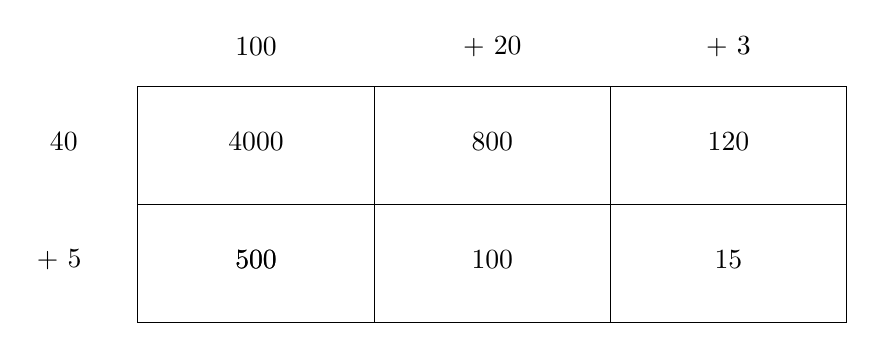
\begin{tikzpicture}
\node at (3.5,0.5) {100};
\node at (6.5,0.5) {+ 20};
\node at (9.5,0.5) {+ 3}; % multiplicand
\node at (1,-0.7) {\ 40};
\node at (1,-2.2) {+ 5}; % multiplier
\draw (2,0) -| (11,-3);
\draw (2,0) |- (11,-3);
\draw (2,-1.5) -- (11,-1.5);
\draw (5,0) -- (5,-3);
\draw (8,0) -- (8,-3); % box & gridlines
\node at (3.5,-0.7) {4000};
\node at (3.5,-2.2) {500};
\node at (6.5,-0.7) {800};
\node at (9.5,-0.7) {120};
\node at (3.5,-2.2) {500};
\node at (6.5,-2.2) {100};
\node at (9.5,-2.2) {15};
\end{tikzpicture}
\\

\begin{center}
\begin{tabular}{c@{\,}c@{\,}c@{\,}c@{\,}c}
^{1}&4&0&0&0\\
	& &8&0&0\\
  + & &1&2&0\\
    & &5&0&0\\
    & &1&0&0\\
  + & & &1&5\\
  	\hline
	&5,&5&3&5\\
	\hline
	\hline
\end{tabular}
\end{center}

\item Using box multiplication, what is $15 \times 7$?
\item Using box multiplication, what is $23 \times 42$?
\item Using box multiplication, what is $17 \times 234$?

\section*{Multiplication in Columns}

\subsection*{Multiplying by a single-digit number}

Start learning to do multiplication in columns by learning to multiply a multi-digit number by a single-digit number.\\

Write the times symbol, with the multiplier under the multiplicand, lined up with the ones-digit, and draw a line under this.\\

Multiply the multiplier by each digit of the multiplicand, starting with the ones digit, and write the products under the line, each lined up under its own column. These are called partial products or sub-products.\\

Draw another line under this and add these partial products to get the product. Draw a double line under this to show that it is the final answer.\\

\begin{center}
\begin{tabular}{c@{\,}c@{\,}c@{\,}c@{\,}c}
      &1,&2&3&4\\
\times & & & &6\\
\cline{1-5}
       & & &2&4\\
    & &^{1}1&8&\\
        &1&2& &\\
      + &6& & &\\
\cline{1-5}
        &7,&4&0&4\\
\hline
\hline
\end{tabular}
\end{center}

\item Multiply 234 by 7, writing down the partial products and adding them up.
\item Multiply 3247 by 3, writing down the partial products and adding them up.

Filling in the blank spaces in the list of partial products with zeroes helps to make sure that your next partial product starts in the right column. It also makes it easier to keep the columns lined up so that it's easier to add up without errors.

\begin{center}
\begin{tabular}{c@{\,}c@{\,}c@{\,}c@{\,}c}
       &1,&2&3&4\\
\times  & & & &6\\
\hline
        & & &2&4\\
    & &^{1}1&8&0\\
        &1&2&0&0\\
      + &6&0&0&0\\
\hline
       &7,&4&0&4\\
\hline
\hline
\end{tabular}\\
\end{center}

\item Multiply 567 by 2, writing down the partial products, padded with zeroes, and adding them up.
\item Multiply 876 by 4, writing down the partial products, padded with zeroes, and adding them up.

You can do this all on one line by doing the carries for the addition at the same time as you are working out the sub-products.

\begin{center}
\begin{tabular}{c@{\,}c@{\,}c@{\,}c@{\,}c}
          &1,&2&3&4\\
\times &_1_&_2&_2&6\\
\hline
          &7,&4&0&4\\
\hline
\hline
\end{tabular}\\
\end{center}

And that's how you multiply any long number by a single-digit number.\\

\item Multiply 35 by 9, writing down the partial products, padded with zeroes, and doing the carries as you write the partial product.
\item Multiply 978 by 4, writing down the partial products, padded with zeroes, and doing the carries as you write the partial product.
\item Multiply 4235 by 8, writing down the partial products, padded with zeroes, and doing the carries as you write the partial product.

\subsection*{Multiplying any two numbers}

Write the times symbol and the multiplier under the multiplicand, with place-values under each other, and draw a line under this. The longer number should be the multiplicand on top.\\

Multiply each digit of the multiplier by each digit of the multiplicand, starting with units.\\

You will get a set of partial products for each digit of the multiplier. Make sure these are all written in their correct column.\\

\begin{center}
\begin{tabular}{c@{\,}c@{\,}c@{\,}c@{\,}c}
       & & &2&3\\
\times & & &3&4\\
\hline
       & & &1&2\\
      +& & &8& \\
\hline
       & & &9& \\
  +& &^{1}6& & \\
\hline
       & &7&8&2\\
\hline
\hline
\end{tabular}\\
\end{center}

\item Multiply 12 by 56, making 2 sets of 2 partial products, and adding them up.
\item Multiply 354 by 32, making 2 sets of 3 partial products, and adding them up.

\vspace{32pt}
Again, pad the blank spaces with zeroes to make it easier to add up without errors.\\

\begin{center}
\begin{tabular}{c@{\,}c@{\,}c@{\,}c@{\,}c}
       & & &2&3\\
\times & & &3&4\\
\hline
       & & &1&2\\
      +& & &8&0\\
\hline
       & & &9&0\\
  +& &^{1}6&0&0\\
\hline
       & &7&8&2\\
\hline
\hline
\end{tabular}\\
\end{center}

\item Multiply 65 by 43, making 2 sets of 2 partial products, padded with zeroes, and adding them up.
\item Multiply 756 by 55, making 2 sets of 3 partial products, padded with zeroes, and adding them up.

This can be shortened by doing the carrying for addition while you're writing the partial products. You will now have only a single partial product for each digit of the multiplier.

\begin{center}
\begin{tabular}{c@{\,}c@{\,}c@{\,}c@{\,}c}
       &&&2&3\\
\times &&&_{1}3&4\\
\hline
       &&&9&2\\
+ &&^{1}6&9&0\\
\hline
      &&7&8&2\\
\hline
\hline
\end{tabular}\\
\end{center}

\vspace{32pt}
And that is how you multiply.\\

\item Multiply 65 by 43, making 2 sets of 2 partial products, padded with zeroes, doing the carries for addition as you write, and adding them up.
\item Multiply 867 by 54, making 2 sets of 3 partial products, padded with zeroes, doing the carries for addition as you write, and adding them up.

Here is longer example:

\begin{center}
\begin{tabular}{c@{\,}c@{\,}c@{\,}c@{\,}c@{\,}c@{\,}c}
       & & & &8&9&7\\
\times & & & &7&8&9\\
\hline
       & & & & &6&3\\
   & & & &^{1}8&1& \\
  +& & &^{2}7&2& & \\
\hline
       & & & &5&6& \\
       & & &7&2& & \\
  +& &^{2}6&4& & & \\
\hline
       & & &4&9& & \\
       & &6&3& & & \\
  +&^{2}5&6& & & & \\
\hline
      &7&0&7,&7&3&3 \\
\hline
\hline
\end{tabular}\\
\end{center}

\vspace{32pt}
See how there are partial products for the units, the tens, and the hundreds of the multiplier, each aligned with its digit of the multiplier.\\

Padding with zeroes makes adding easier and prevents errors by keeping columns in line.

\begin{center}
\begin{tabular}{c@{\,}c@{\,}c@{\,}c@{\,}c@{\,}c@{\,}c}
       & & & &8&9&7\\
\times & & & &7&8&9\\
\hline
       & & & & &6&3\\
   & & & &^{1}8&1&0\\
  +& & &^{2}7&2&0&0\\
\hline
       & & & &5&6&0\\
       & & &7&2&0&0\\
  +& &^{2}6&4&0&0&0\\
\hline
       & & &4&9&0&0\\
       & &6&3&0&0&0\\
  +&^{2}5&6&0&0&0&0\\
\hline
      &7&0&7,&7&3&3\\
\hline
\hline
\end{tabular}\\
\end{center}

\vspace{32pt}
You can make this shorter by doing carries while working out the partial products. Here padding with zeroes just reminds you where to write the partial products. This is the usual way to do multiplication of large numbers by hand.

\begin{center}
\begin{tabular}{c@{\,}c@{\,}c@{\,}c@{\,}c@{\,}c@{\,}c}
           &&&&8&9&7\\
    \times &&&&7&8&9\\
  _6&_4&_7&_5&_8&_6&\\
\hline
  &&&^{1}8&^{1}0&7&3\\
     &&^{1}7&1&7&6&0\\
    &^{1}6&2&7&9&0&0\\
\hline
       &7&0&7,&7&3&3\\
\hline
\hline
\end{tabular}\\
\end{center}

\item (Optional challenge!) Multiply 764 by 345.

\subsection*{Multiplication with Decimal Fractions}

In doing multiplication of decimal fractions in columns, first fill with trailing zeroes so that both numbers have the same number of digits after the decimal point, so that the columns are aligned properly. Then you can do the multiplication the same as for whole numbers and work out where to put the decimal point when you're done.\\

The number of digits after the decimal point of the product is the total of the number of digits after the decimal point of the multiplicand and of the multiplier.\\

\begin{center}
\begin{tabular}{c@{\,}c@{\,}c@{\,}c@{\,}c@{\,}c@{\,}c@{\,}c@{\,}c@{\,}c@{\,}}
       & & & & & &2&.&3&4\\
\times & & & & & &5&.&2&0\\
\hline
       & & & & & & & & &0\\
       & & & & & & & &0& \\
+      & & & & & &0& & & \\
\hline
       & & & & & & & &8& \\
       & & & & & &6& & & \\
+      & & & &4& & & & & \\
\hline
       & & & &2& &0& & & \\
   & &^{1}1& &5& & & & & \\
+      &1&0& & & & & & & \\
\hline
       &1&2&.&1& &6& &8&0\\
\hline
\hline
\end{tabular}\\
\end{center}

Padding the partial products with zeroes makes the columns easier to see and can prevent errors, and you don't actually  need to multiply out the first zero.

\begin{center}
\begin{tabular}{c@{\,}c@{\,}c@{\,}c@{\,}c@{\,}c@{\,}c@{\,}c@{\,}c@{\,}c@{\,}}
       & & & & & &2&.&3&4\\
\times & & & & & &5&.&2&0\\
\hline
       & & & & & & & &8&0\\
       & & & & & &6& &0&0\\
+      & & & &4& &0& &0&0\\
\hline
       & & & &2& &0& &0&0\\
   & &^{1}1& &5& &0& &0&0\\
+      &1&0& &0& &0& &0&0\\
\hline
       &1&2&.&1& &6& &8&0\\
\hline
\hline
\end{tabular}\\
\end{center}

\vspace{32pt}
You can make this even shorter if you do carries while working out the partial products, and you don't really need to add the trailing zero to the multiplier as long as the decimal points line up.

\begin{center}
\begin{tabular}{c@{\,}c@{\,}c@{\,}c@{\,}c@{\,}c@{\,}c@{\,}c@{\,}c@{\,}c@{\,}}
       & & & & & &2&.&3&4\\
\times & &_1& &_2& &5&.&2& \\
\hline
       & & & &4& &6& &8& \\
  +&1&^{1}1& &7& &0& &0& \\
\hline
       &1&2&.&1& &6& &8& \\
\hline
\hline
\end{tabular}\\
\end{center}

\item Multiply 3.1 by 3.2
\item Multiply 0.65 by 3.2
\item Multiply 12 by 4.5
\item Multiply 3.17 by 6.8
\item Multiply 8.3 by 3

\section*{Checking Multiplication}

\paragraph{Reversing Order}
You can check the result of your multiplication by reversing the multiplicand and multiplier to verify that they both give the same product.\\

\begin{center}
\begin{tabular}{c@{\,}c@{\,}c@{\,}c@{\,}c}
       &&&2&3\\
\times &&&_{1}4&2\\
\hline
       &&&4&6\\
     + &&9&2&0\\
\hline
       &&9&6&6\\
\hline
\hline
\end{tabular}\\
\end{center}
\begin{center}
\begin{tabular}{c@{\,}c@{\,}c@{\,}c@{\,}c}
       &&&4&2\\
\times &&&2&3\\
\hline
       &&1&2&6\\
     + &&8&4&0\\
\hline
       &&9&6&6\\
\hline
\hline
\end{tabular}
\end{center}

\begin{center}
$23 \times 42$ should equal $42 \times 23$.\ \ding{51}\\
\end{center}

\item Multiply 32 by 67. Now check you answer by multiplying 67 by 32. Did you get it right?

\paragraph{Casting Out 9s}

\begin{center}
\begin{tabular}{c@{\,}c@{\,}c@{\,}c@{\,}c}
       &&&2&3\\
\times &&&_{1}4&2\\
\hline
       &&&4&6\\
     + &&9&2&0\\
\hline
       &&9&6&6\\
\hline
\hline
\end{tabular}\\
\end{center}

The digit sums of the factors, multiplied, should equal the digit sum of the product.\\

\begin{center}
\begin{align*}
2 + 3 &= 5\\
4 + 2 &= 6\\\\
\cancel{9} + 6 + 6 &= 12; 1 + 2 = 3\\
5 \times 6 &= 30; 3 + 0 = 3\\
\end{align*}
\ding{51}
\end{center}

\item Multiply 87 by 32. Now check your answer by casting out 9s and working out the digit sums. Did you get it right?

\end{enumerate}

\end{document}